\documentclass[a4paper]{article}
\usepackage{graphicx}
\usepackage{amsmath}
\usepackage{caption}
\usepackage{subcaption}
\usepackage{nth}[super]

%\floatstyle{boxed}
%\restylefloat{figure}
\begin{document}

\centerline{\sc \large APPENDIX A}
\vspace{.5pc}
\centerline{\sc Genetic Algorithm Implementation and testing in C++}
\vspace{2pc}

\section{Background}
The standard genetic algorithm constructed using selection, crossover and mutation over successive generations is implemented using the C++ programming language. The choice of C++ over the standard engineering programming tool, \verb!MATLAB!, is justified by the need for quick computations and reduced running time in light of the large number of computations that are involved in the solution of the target optimisation problem. \\

While the algorithm has earlier been implemented and tested in \verb!MATLAB!, the object oriented structure that C++ necessitates lends a more complete and integrated solution structure when combined with the propulsion optimisation problem at hand. To begin with, a simple genetic algorithm was constructed in C++ in a manner so as to insulate the algorithm engine from the function to be optimised. This renders a generic solver that can later be adapted to specific optimisation problems. The so-constructed algorithm was first tested using three standard benchmark functions that are used to evaluate the performance of optimisation schemes in the literature:
\begin{itemize}
\item Goldstein Price Function
\item Beale's Function
\item Booth's function
\end{itemize}

The minimas of the three functions listed above were verified using the algorithm and the solution code was thus tested to be reliable and consistent across repeated refreshed runs of the algorithm.\\

\section{Algorithm performance for benchmark functions}

Standard two-dimensional functions are used to benchmark optimisation schemes and validate the optimas indicated by the scheme at hand. A similar mode of evaluation is employed here and the convergence of the population to the optima in each case tracked. In addition, the fitness of the fittest individual in each generation and the convergence of the best fitness with increasing generation number is observed. Below are plots of the population and fitness over 500 generations, each consisting of 30 individuals.\\ 

\subsection{Goldstein Price Function}

The Goldstein Price function in 2 variables is given by:
%\begin{equation}
\begin{multline}
f(x,y)=(1+(x+y+1)^2(19-14x+3x^2-14y+6xy+3y^2))\\
	(30+(2x-3y)^2(18-32x+12x^2+48y-36xy+27y^2))
\end{multline}
%\end{equation}

The minima of the Goldstein Price function lies at (x,y)=(0,-1) and the function value at the minima is -3. This is verified by the algorithm outputs.

\begin{figure}[hb!]
\centering
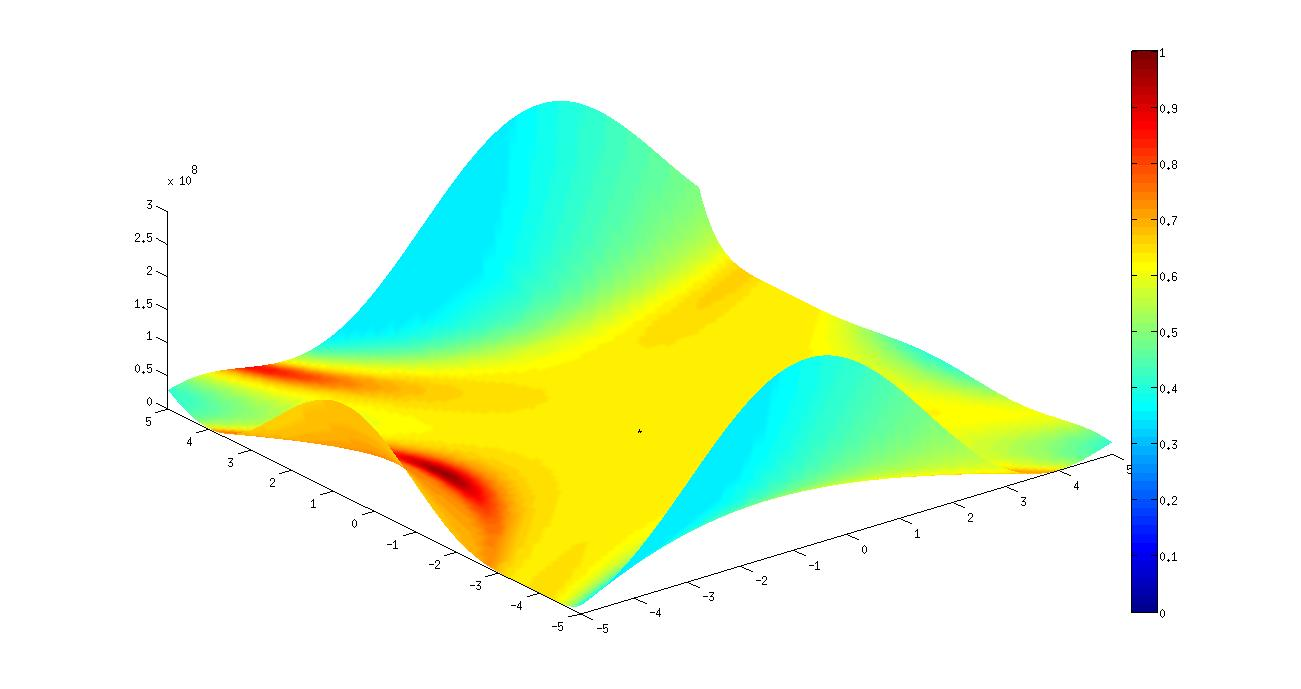
\includegraphics[width=\textwidth]{GPR.jpg}
\caption{Goldstein Price Function}
\label{GPR}
\end{figure}

\begin{figure}[hb!]
\centering
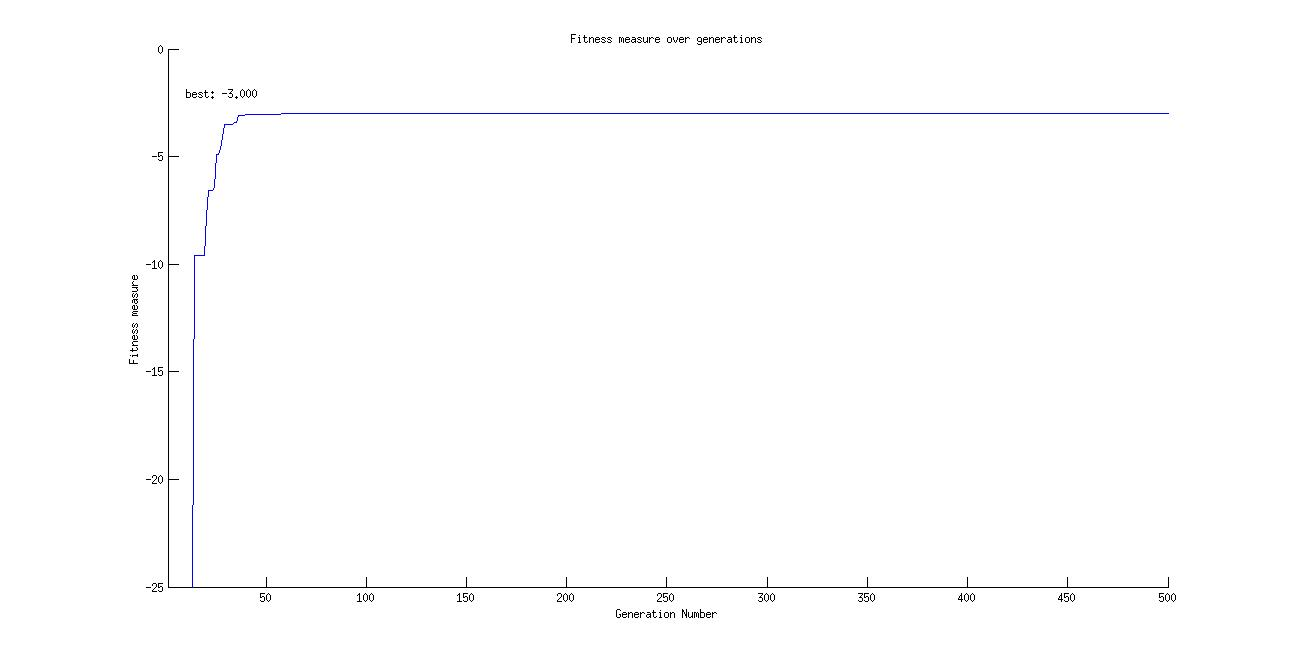
\includegraphics[width=\textwidth]{GPR_fitness_vs_generation.jpg}
\caption{Progress of population best fitness over generations, Goldstein Price Function}
\label{GPRF}
\end{figure}

\begin{figure}[ht!]
\begin{subfigure}[b]{0.5\textwidth}
\centering
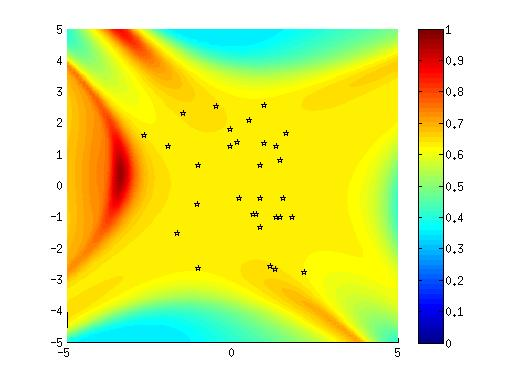
\includegraphics[width=\textwidth]{GPR1.jpg}
\caption{\centerline{\nth{1} generation\\ Goldstein Price Function}}
\label{GPR1}
\end{subfigure}
\quad
\begin{subfigure}[b]{0.5\textwidth}
\centering
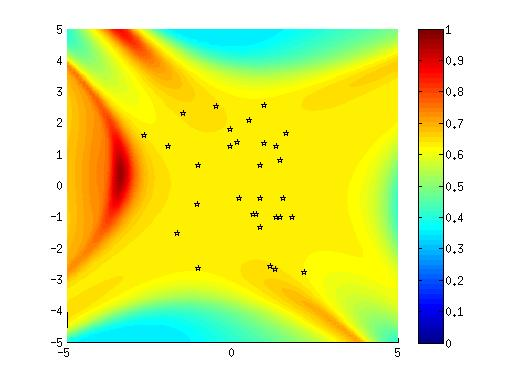
\includegraphics[width=\textwidth]{GPR2.jpg}
\caption{\centerline{\nth{3} generation\\ Goldstein Price Function}}
\label{GPR2}
\end{subfigure}

\begin{subfigure}[b]{0.5\textwidth}
\centering
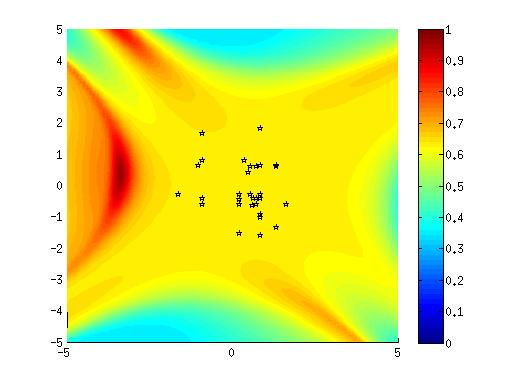
\includegraphics[width=\textwidth]{GPR4.jpg}
\caption{\centerline{\nth{5} generation\\ Goldstein Price Function}}
\label{GPR3}
\end{subfigure}
\quad
\begin{subfigure}[b]{0.5\textwidth}
\centering
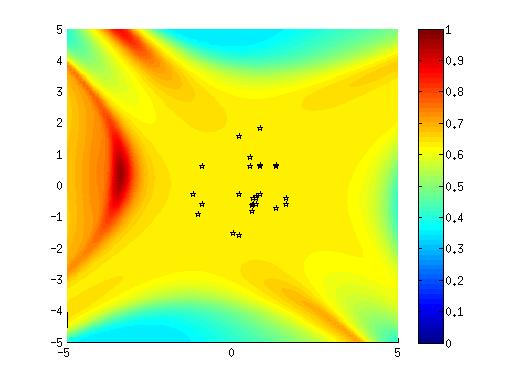
\includegraphics[width=\textwidth]{GPR5.jpg}
\caption{\centerline{\nth{9} generation\\ Goldstein Price Function}}
\label{GPR4}
\end{subfigure}

\begin{subfigure}[b]{0.5\textwidth}
\centering
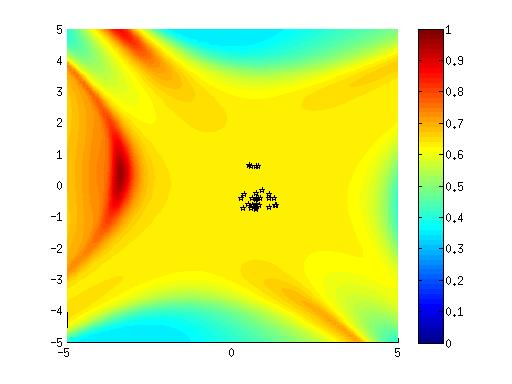
\includegraphics[width=\textwidth]{GPR7.jpg}
\caption{\centerline{\nth{10} generation\\ Goldstein Price Function}}
\label{GPR5}
\end{subfigure}
\quad
\begin{subfigure}[b]{0.5\textwidth}
\centering
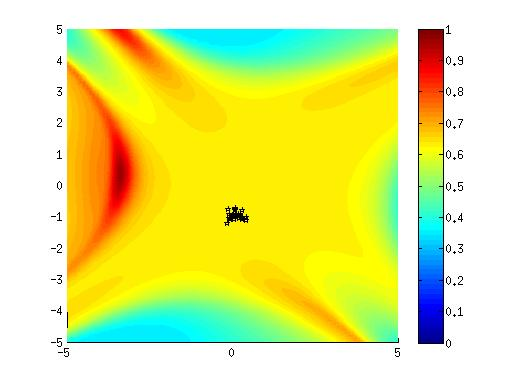
\includegraphics[width=\textwidth]{GPR9.jpg}
\caption{\centerline{Final generation\\ Goldstein Price Function}}
\label{GPR6}
\end{subfigure}
\caption{Convergence of populations over generations, Goldstein Price Function}
\label{GPRT}
\end{figure}

\clearpage

\subsection{Beale's function}

Beale's function is defined by:
\begin{equation}
f(x,y) = (1.5-x+xy)^2+(2.25-x+xy^2)^2+(2.625-x+xy^3)^2
\end{equation}
The function has a minimum value of 0 at $(3,0.5)$.

\begin{figure}[hb!]
\centering
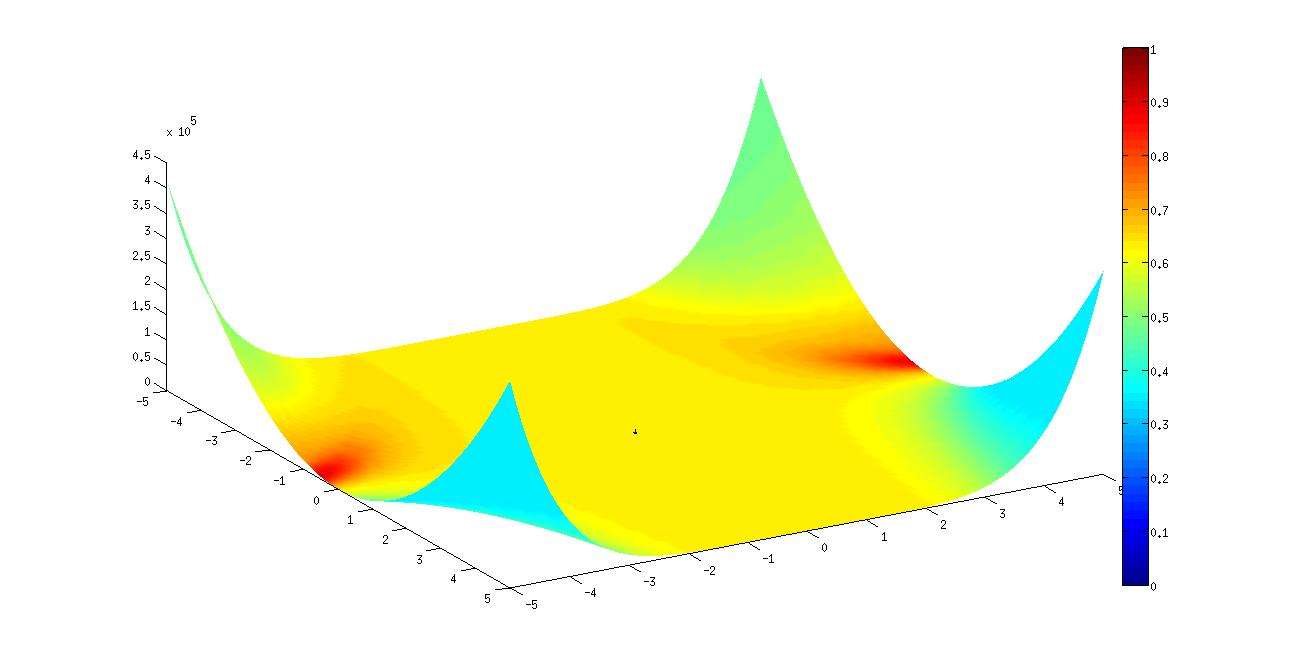
\includegraphics[width=\textwidth]{Beale.jpg}
\caption{Beale's function}
\label{B1}
\end{figure}

\begin{figure}[hb!]
\centering
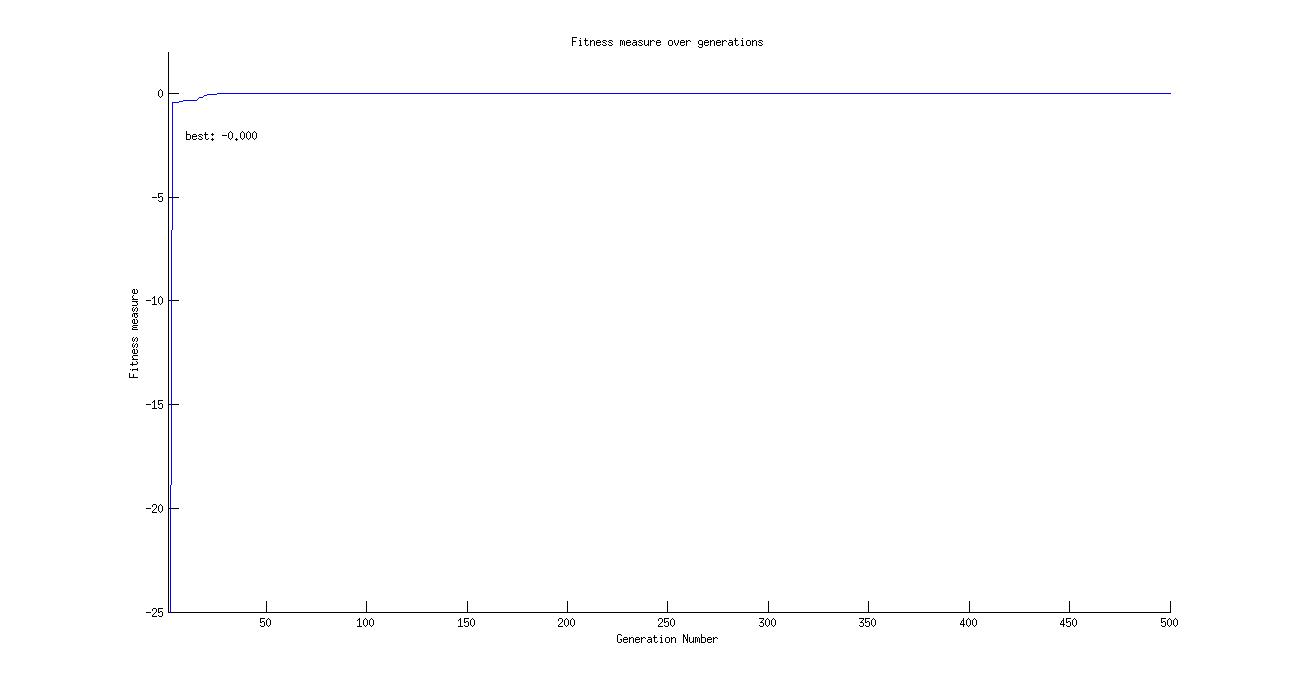
\includegraphics[width=\textwidth]{Beale_fitness_vs_generation.jpg}
\caption{Progress of population best fitness over generations, Beale's function}
\label{B1F}
\end{figure}

\begin{figure}
\begin{subfigure}[b]{0.5\textwidth}
\centering
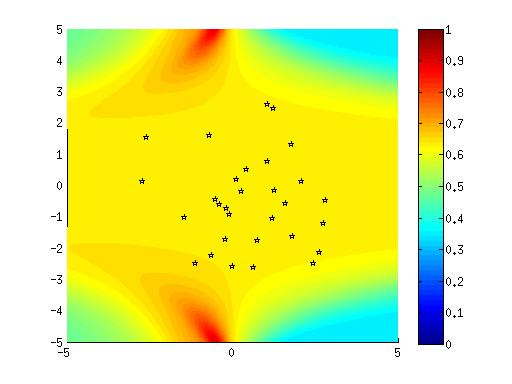
\includegraphics[width=\textwidth]{Beale1.jpg}
\caption{\centerline{\nth{1} generation\\ Beale's Function}}
\label{B11}
\end{subfigure}
\quad
\begin{subfigure}[b]{0.5\textwidth}
\centering
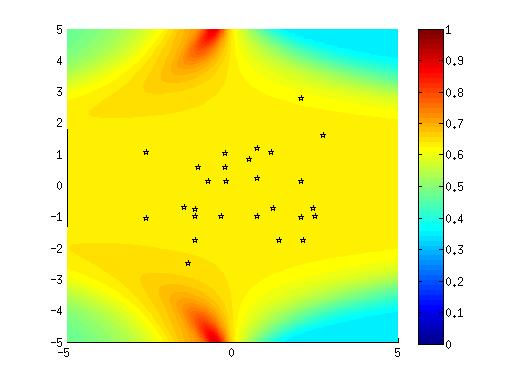
\includegraphics[width=\textwidth]{Beale2.jpg}
\caption{\centerline{\nth{3} generation\\ Beale's Function}}
\label{B12}
\end{subfigure}

\begin{subfigure}[b]{0.5\textwidth}
\centering
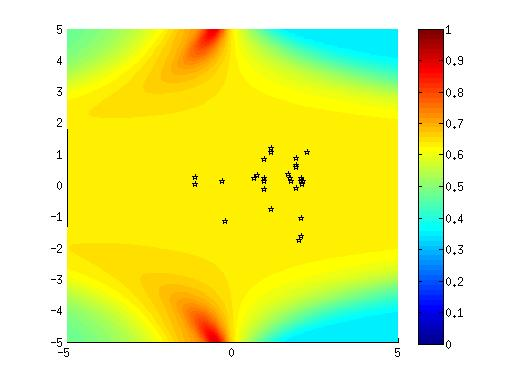
\includegraphics[width=\textwidth]{Beale4.jpg}
\caption{\centerline{\nth{5} generation\\ Beale's Function}}
\label{B13}
\end{subfigure}
\quad
\begin{subfigure}[b]{0.5\textwidth}
\centering
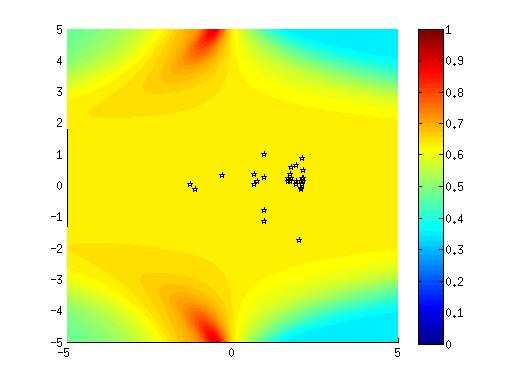
\includegraphics[width=\textwidth]{Beale5.jpg}
\caption{\centerline{\nth{9} generation\\ Beale's Function}}
\label{B14}
\end{subfigure}

\begin{subfigure}[b]{0.5\textwidth}
\centering
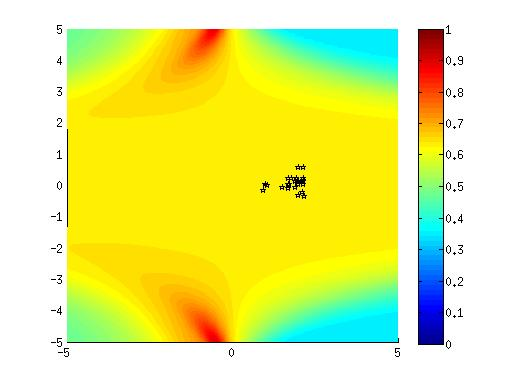
\includegraphics[width=\textwidth]{Beale7.jpg}
\caption{\centerline{\nth{10} generation\\ Beale's Function}}
\label{B15}
\end{subfigure}
\quad
\begin{subfigure}[b]{0.5\textwidth}
\centering
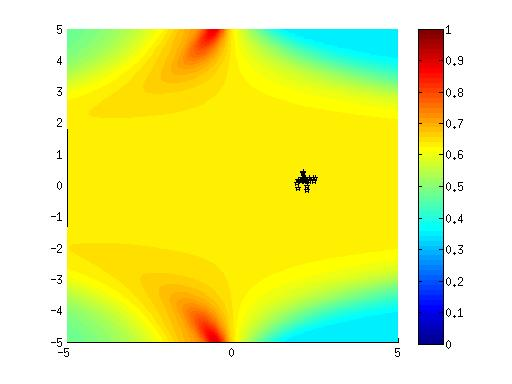
\includegraphics[width=\textwidth]{Beale9.jpg}
\caption{\centerline{Final generation\\ Beale's Function}}
\label{B16}
\end{subfigure}
\caption{Convergence of populations over generations, Beale's function}
\label{Beale}
\end{figure}

\clearpage

\subsection{Booth's function}

Booth's function is defined as:
\begin{equation}
f(x,y)=(x+2y-7)^2+(2x+y-5)^2
\end{equation}
The function has a minima of 0 at $(1,3)$.

\begin{figure}[hb!]
\begin{subfigure}[b]{0.5\textwidth}
\centering
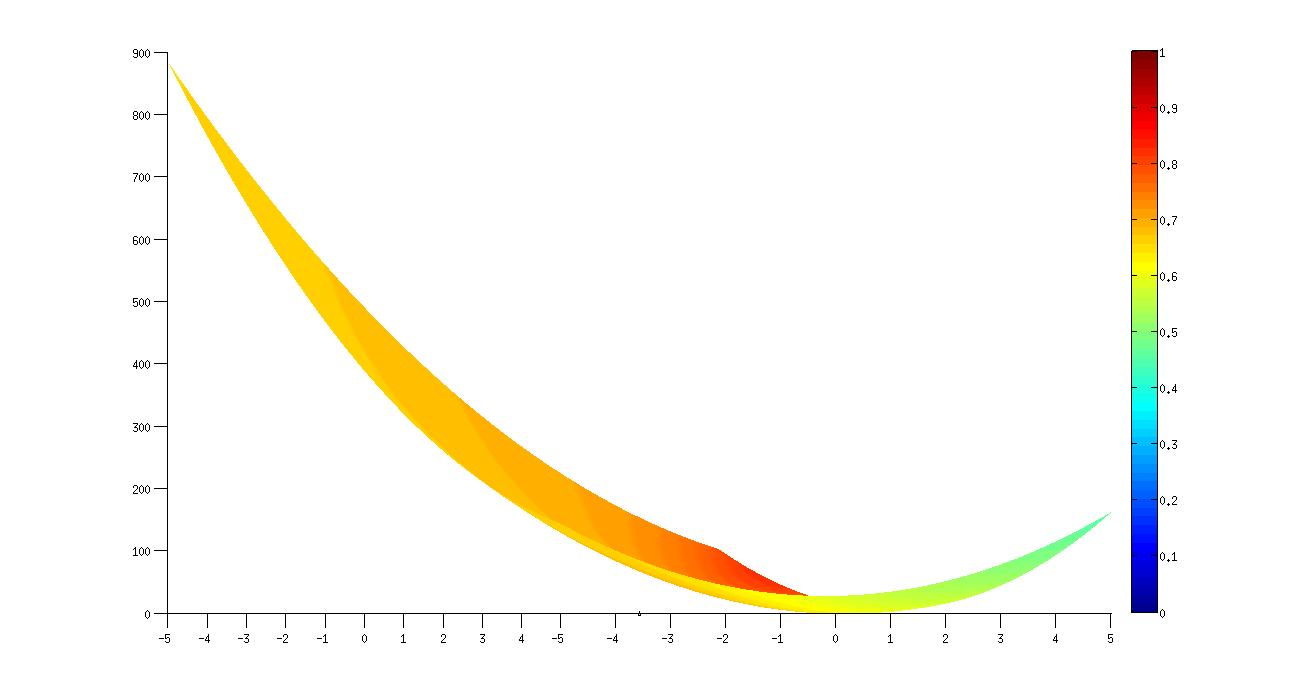
\includegraphics[width=1.2\textwidth]{BoothA.jpg}
\caption{Booth's Function (A)}
\label{B2A}
\end{subfigure}
\quad
\begin{subfigure}[b]{0.5\textwidth}
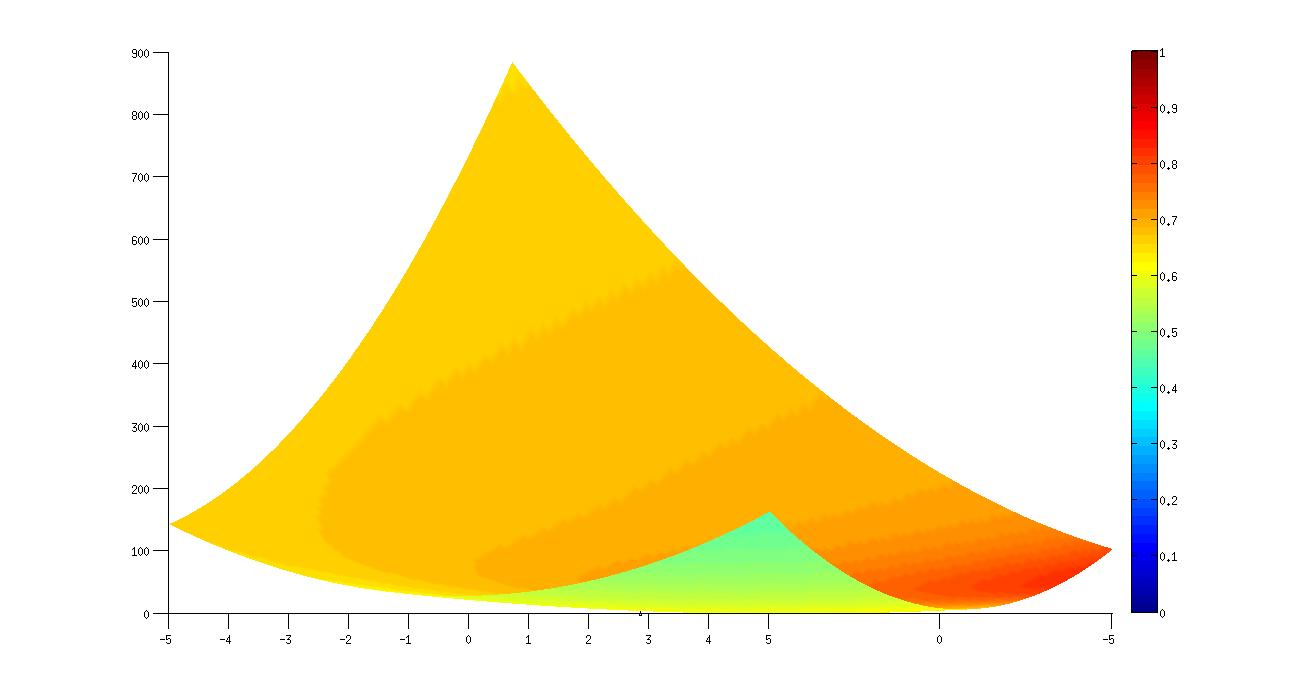
\includegraphics[width=1.2\textwidth]{BoothB.jpg}
\caption{Booth's Function (B)}
\label{B2B}
\end{subfigure}
\caption{Booth's function}
\label{B2}
\end{figure}

\begin{figure}[hb!]
\centering
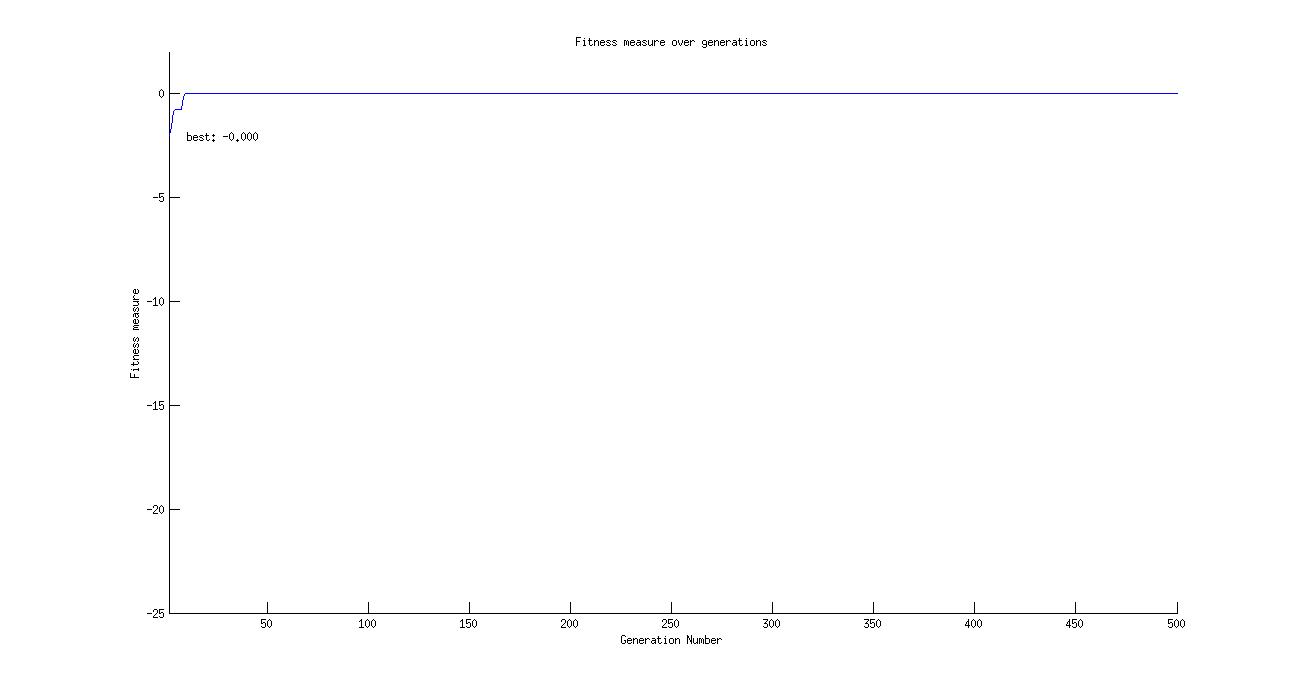
\includegraphics[width=\textwidth]{Booth_fitness_vs_generation.jpg}
\caption{Progress of population best fitness over generations, Booth's function}
\label{B2F}
\end{figure}

\begin{figure}
\begin{subfigure}[b]{0.5\textwidth}
\centering
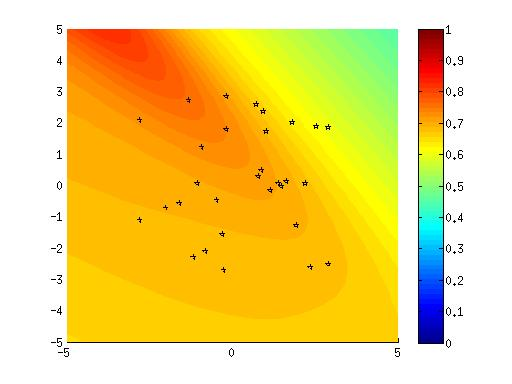
\includegraphics[width=\textwidth]{Booth1.jpg}
\caption{\centerline{\nth{1} generation\\ Booth's Function}}
\label{B21}
\end{subfigure}
\quad
\begin{subfigure}[b]{0.5\textwidth}
\centering
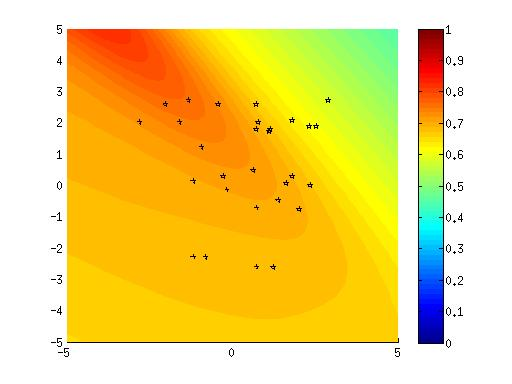
\includegraphics[width=\textwidth]{Booth2.jpg}
\caption{\centerline{\nth{3} generation\\ Booth's Function}}
\label{B22}
\end{subfigure}

\begin{subfigure}[b]{0.5\textwidth}
\centering
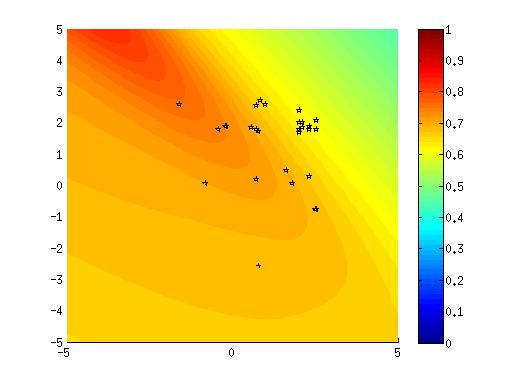
\includegraphics[width=\textwidth]{Booth4.jpg}
\caption{\centerline{\nth{5} generation\\ Booth's Function}}
\label{B23}
\end{subfigure}
\quad
\begin{subfigure}[b]{0.5\textwidth}
\centering
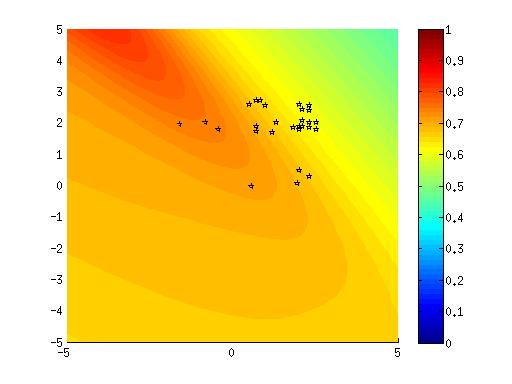
\includegraphics[width=\textwidth]{Booth5.jpg}
\caption{\centerline{\nth{9} generation\\ Booth's Function}}
\label{B24}
\end{subfigure}

\begin{subfigure}[b]{0.5\textwidth}
\centering
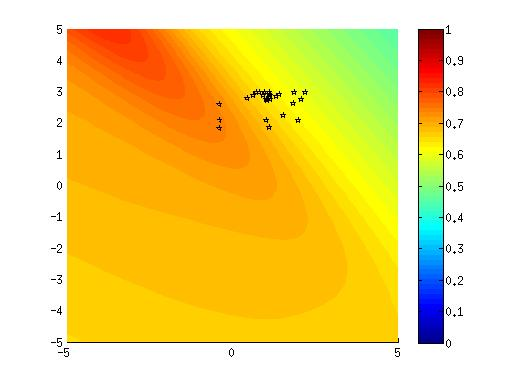
\includegraphics[width=\textwidth]{Booth7.jpg}
\caption{\centerline{\nth{10} generation\\ Booth's Function}}
\label{B25}
\end{subfigure}
\quad
\begin{subfigure}[b]{0.5\textwidth}
\centering
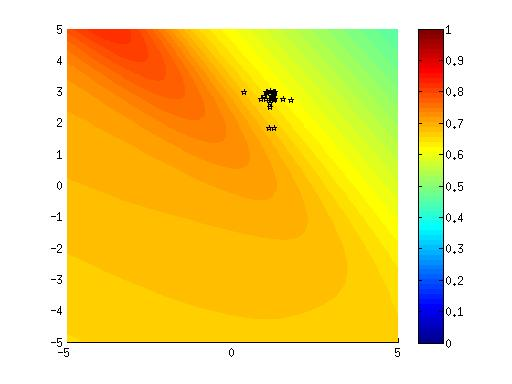
\includegraphics[width=\textwidth]{Booth9.jpg}
\caption{\centerline{Final generation\\ Booth's Function}}
\label{B26}
\end{subfigure}
\caption{Convergence of populations over generations, Booth's function}
\label{Booth}
\end{figure}

\clearpage

\listoffigures
\end{document}
